\documentclass[tikz, border=5mm]{standalone}
\usepackage{amsmath}
 \usetikzlibrary{arrows.meta,decorations.markings}
\usetikzlibrary{intersections, backgrounds, calc, patterns}

\begin{document}
% Preamble:
% \usepackage{tikz}
% \usetikzlibrary{arrows.meta,decorations.markings,calc}

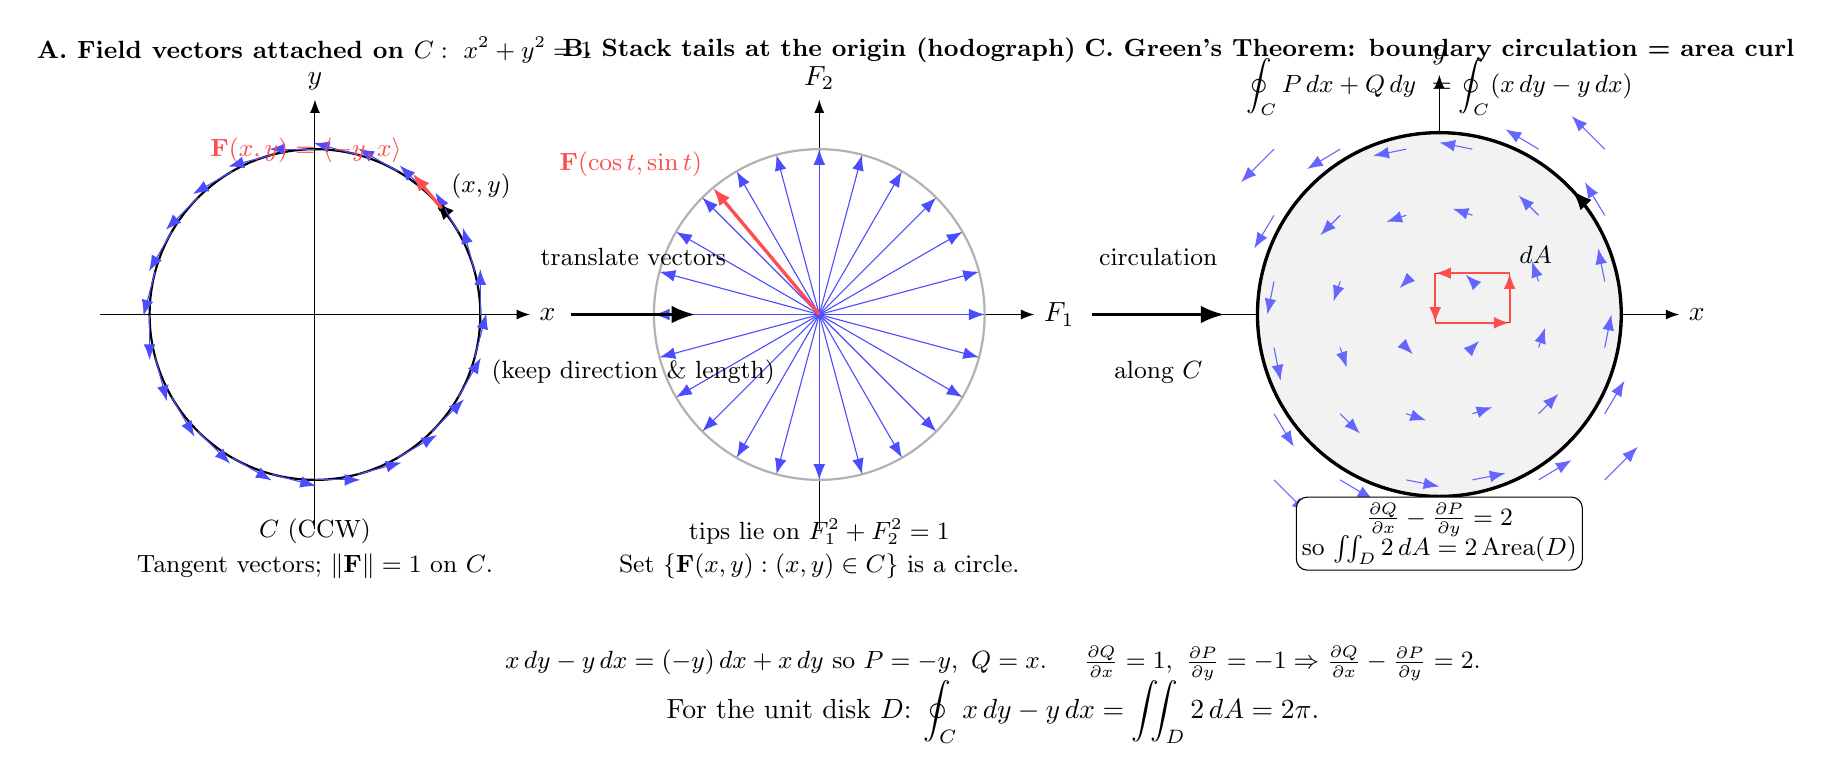
\begin{tikzpicture}[>=Latex,scale=1.05]
	
	% ======================================================
	% Panel A: Vectors attached along the unit circle C
	% ======================================================
	\begin{scope}[shift={(-8.2,0)}]
		\node[align=center] at (0,3.2)
		{\small \textbf{A. Field vectors attached on }$C:\ x^2+y^2=1$};
		
		% Axes
		\draw[->] (-2.6,0) -- (2.6,0) node[right] {$x$};
		\draw[->] (0,-2.6) -- (0,2.6) node[above] {$y$};
		
		% Unit circle C with positive orientation
		\draw[thick,
		postaction={decorate},
		decoration={markings, mark=at position 0.12 with {\arrow{Latex[length=2.4mm]}}}
		] (0,0) circle (2.0);
		\node[below] at (0,-2.35) {\small $C$ (CCW)};
		
		% Vector field F(x,y)=<-y,x> along C
		\def\arrowlen{0.55}
		\foreach \ang in {0,15,...,345}{
			\coordinate (P) at ({2.0*cos(\ang)},{2.0*sin(\ang)});
			\draw[blue!70, -{Latex[length=2.0mm]}]
			(P) -- ++({\arrowlen*(-sin(\ang))},{\arrowlen*(cos(\ang))});
		}
		
		% One highlighted point
		\coordinate (Ph) at ({2.0*cos(40)},{2.0*sin(40)});
		\fill (Ph) circle (1.2pt);
		\node[above right] at (Ph) {\small $(x,y)$};
		\draw[red!70, very thick, -{Latex[length=2.3mm]}]
		(Ph) -- ++({\arrowlen*(-sin(40))},{\arrowlen*(cos(40))})
		node[above left] {\small $\mathbf F(x,y)=\langle -y,x\rangle$};
		
		\node[align=center] at (0,-3.05) {\small
			Tangent vectors; \(\|\mathbf F\|=1\) on \(C\).};
	\end{scope}
	
	% ======================================================
	% Panel B: Translate all tails to a single point (hodograph)
	% ======================================================
	\begin{scope}[shift={(-2.1,0)}]
		\node[align=center] at (0,3.2)
		{\small \textbf{B. Stack tails at the origin (hodograph)}};
		
		% Axes
		\draw[->] (-2.6,0) -- (2.6,0) node[right] {$F_1$};
		\draw[->] (0,-2.6) -- (0,2.6) node[above] {$F_2$};
		
		% Circle traced by tips of F on C
		\draw[thick,gray!60] (0,0) circle (2.0);
		\node[below] at (0,-2.35) {\small tips lie on $F_1^2+F_2^2=1$};
		
		% Draw vectors with common tail at origin
		\foreach \ang in {0,15,...,345}{
			\draw[blue!70, -{Latex[length=2.0mm]}]
			(0,0) -- ({2.0*(-sin(\ang))},{2.0*(cos(\ang))});
		}
		
		% Highlight one
		\draw[red!70, very thick, -{Latex[length=2.3mm]}]
		(0,0) -- ({2.0*(-sin(40))},{2.0*(cos(40))})
		node[above left] {\small $\mathbf F(\cos t,\sin t)$};
		
		\node[align=center] at (0,-3.05) {\small
			Set \(\{\mathbf F(x,y):(x,y)\in C\}\) is a circle.};
	\end{scope}
	
	% Arrow between A and B
	\draw[very thick, -{Latex[length=3mm]}] (-5.1,0) -- (-3.6,0);
	\node[align=center] at (-4.35,0.7) {\small translate vectors};
	\node[align=center] at (-4.35,-0.7) {\small (keep direction \& length)};
	
	% ======================================================
	% Panel C: Green's Theorem picture (boundary vs area)
	% ======================================================
	\begin{scope}[shift={(5.4,0)}]
		\node[align=center] at (0,3.2)
		{\small \textbf{C. Green's Theorem: boundary circulation = area curl}};
		
		% Axes
		\draw[->] (-2.9,0) -- (2.9,0) node[right] {$x$};
		\draw[->] (0,-2.9) -- (0,2.9) node[above] {$y$};
		
		% Unit disk D and boundary C
		\fill[gray!10] (0,0) circle (2.2);
		\draw[thick] (0,0) circle (2.2);
		
		% Positive orientation
		\draw[very thick,
		postaction={decorate},
		decoration={markings, mark=at position 0.12 with {\arrow{Latex[length=2.6mm]}}}
		] (0,0) circle (2.2);
		
		% Vector field inside (coarser grid)
		\foreach \x in {-2,-1.2,-0.4,0.4,1.2,2}{
			\foreach \y in {-2,-1.2,-0.4,0.4,1.2,2}{
				\pgfmathsetmacro{\r}{sqrt((\x)^2+(\y)^2)}
				\ifdim \r pt > 0.35pt
				\pgfmathsetmacro{\s}{0.20}
				\pgfmathsetmacro{\vx}{-\s*(\y)}
				\pgfmathsetmacro{\vy}{ \s*(\x)}
				\draw[blue!60,-{Latex[length=2mm]}] (\x,\y) -- ++(\vx,\vy);
				\fi
			}
		}
		
		% Small area element dA + local loop
		\coordinate (A) at (0.4,0.2);
		\draw[black] ($(A)+(-0.45,-0.30)$) rectangle ++(0.90,0.60);
		\node[above right] at ($(A)+(0.45,0.30)$) {\small $dA$};
		\draw[red!70,thick,-{Latex[length=2mm]}] ($(A)+(-0.45,-0.30)$) -- ($(A)+(0.45,-0.30)$);
		\draw[red!70,thick,-{Latex[length=2mm]}] ($(A)+(0.45,-0.30)$) -- ($(A)+(0.45,0.30)$);
		\draw[red!70,thick,-{Latex[length=2mm]}] ($(A)+(0.45,0.30)$) -- ($(A)+(-0.45,0.30)$);
		\draw[red!70,thick,-{Latex[length=2mm]}] ($(A)+(-0.45,0.30)$) -- ($(A)+(-0.45,-0.30)$);
		
		% Curl value = 2
		\node[draw,rounded corners,fill=white,inner sep=2pt,align=center] at (0,-2.65)
		{\small $\frac{\partial Q}{\partial x}-\frac{\partial P}{\partial y}=2$\\[-1pt]
			\small so \(\iint_D 2\,dA=2\,\text{Area}(D)\)};
		
		% Boundary integral label
		\node[align=center] at (0,2.75) {\small
			\(\displaystyle \oint_C P\,dx+Q\,dy\)
			\;=\;\(\displaystyle \oint_C (x\,dy-y\,dx)\)};
	\end{scope}
	
	% Arrow from hodograph to Green panel
	\draw[very thick, -{Latex[length=3mm]}] (1.2,0) -- (2.8,0);
	\node[align=center] at (2.0,0.7) {\small circulation};
	\node[align=center] at (2.0,-0.7) {\small along $C$};
	
	% ======================================================
	% Bottom algebra summary (matches your derivation)
	% ======================================================
	\node[align=center] at (0,-4.6) {\small
		\(x\,dy-y\,dx = (-y)\,dx + x\,dy\) so \(P=-y,\ Q=x\). \quad
		\(\frac{\partial Q}{\partial x}=1,\ \frac{\partial P}{\partial y}=-1\Rightarrow
		\frac{\partial Q}{\partial x}-\frac{\partial P}{\partial y}=2.\)\\[-1pt]
		For the unit disk \(D\): \(\displaystyle \oint_C x\,dy-y\,dx=\iint_D 2\,dA=2\pi.\)};
	
\end{tikzpicture}


\end{document}